\documentclass[newpage]{homework}
\newcommand{\hwname}{Zooey Nguyen}
\newcommand{\hwemail}{zooeyn@ucla.edu}
\newcommand{\hwclass}{Homework Code}
\newcommand{\hwtype}{3}
\newcommand{\hwnum}{}
\begin{document}
\maketitle

\question
Output for Newton's method.
\begin{figure}[htbp]
	\centering
	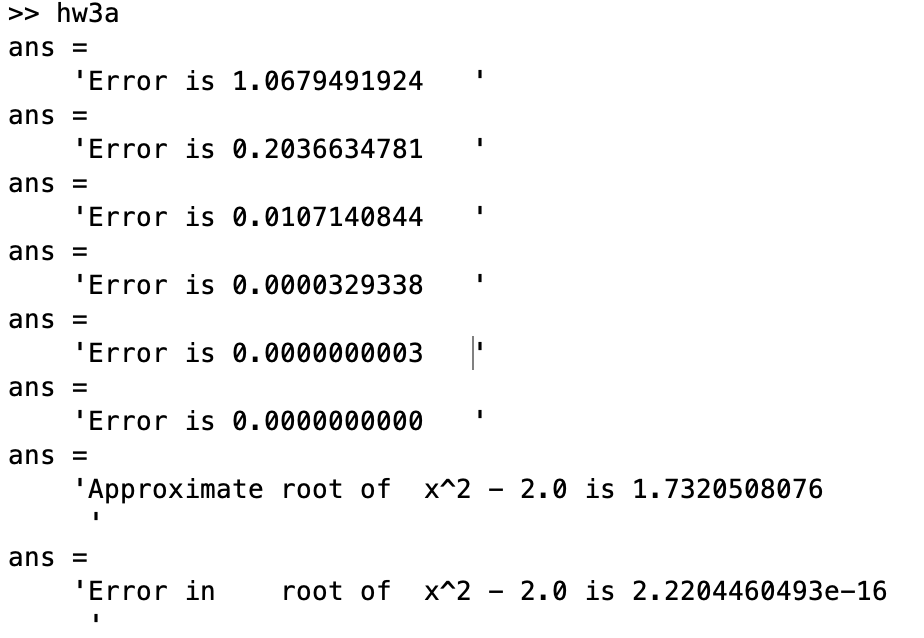
\includegraphics[width=0.8\textwidth]{3a.png}
\end{figure}

\question
Output for modified Newton's method.
\begin{figure}[htbp]
	\centering
	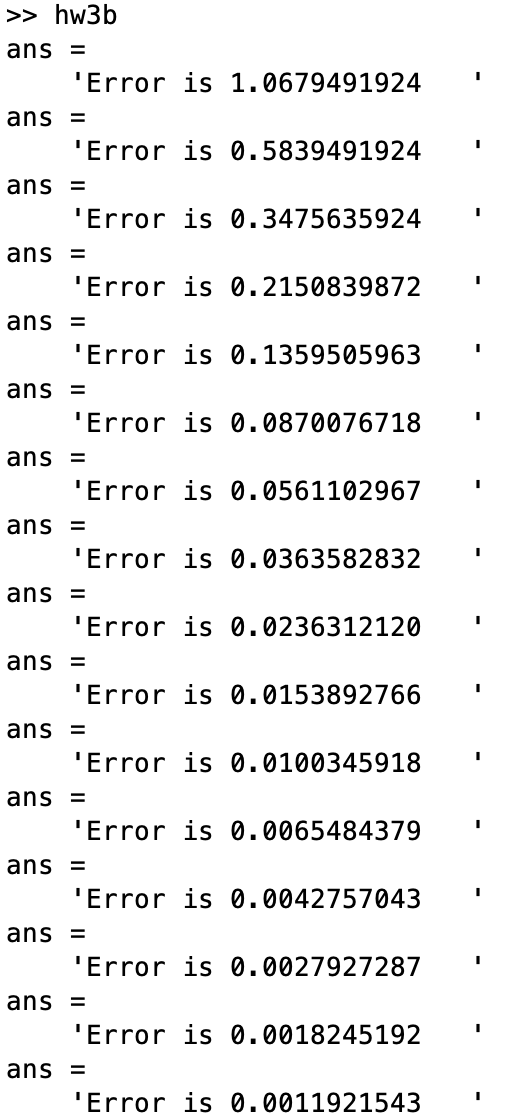
\includegraphics[width=0.5\textwidth]{3bi.png}
\end{figure}

\begin{figure}[htbp]
	\centering
	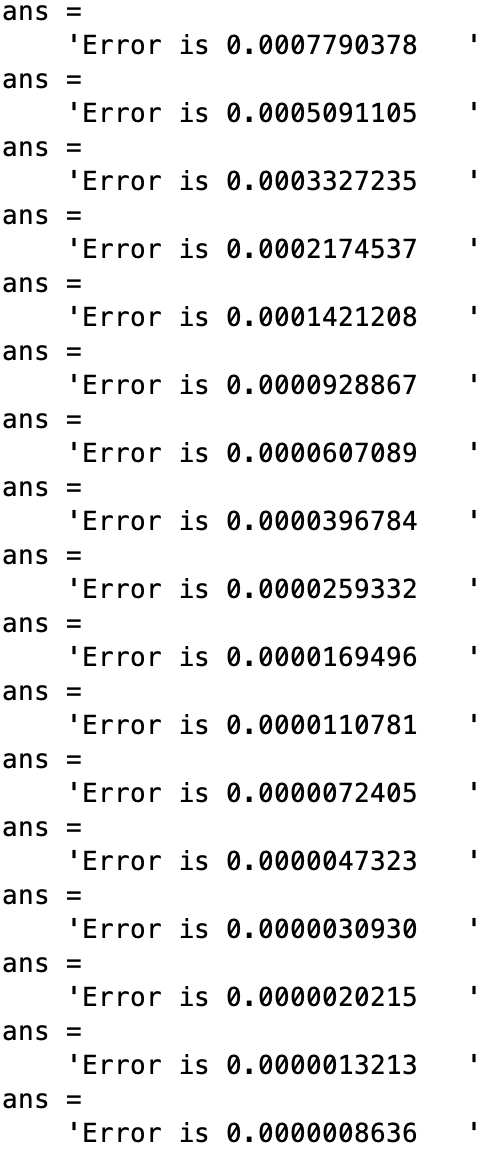
\includegraphics[width=0.5\textwidth]{3bii.png}
\end{figure}

\begin{figure}[htbp]
	\centering
	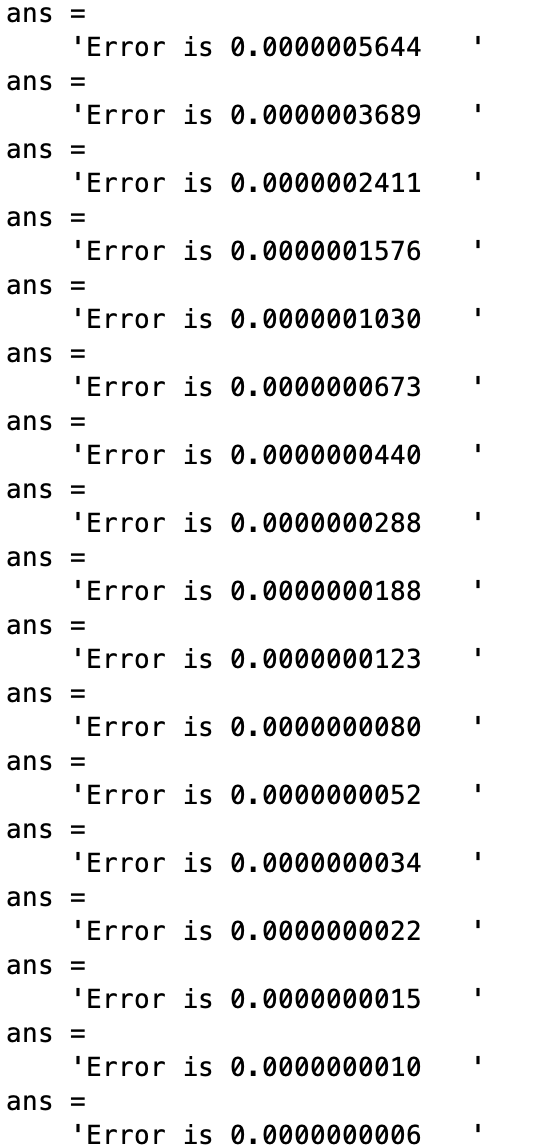
\includegraphics[width=0.5\textwidth]{3biii.png}
\end{figure}

\begin{figure}[htbp]
	\centering
	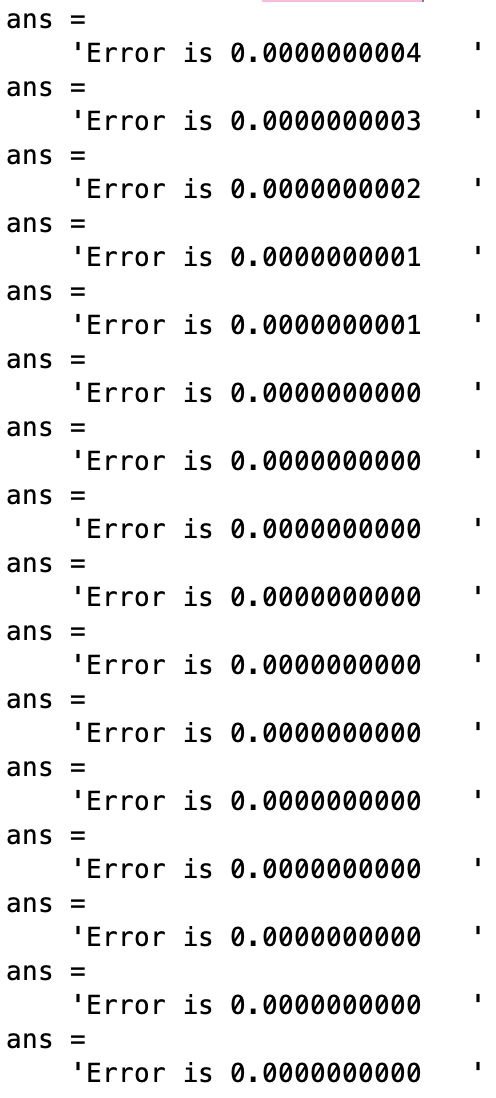
\includegraphics[width=0.5\textwidth]{3biv.png}
\end{figure}

\begin{figure}[htbp]
	\centering
	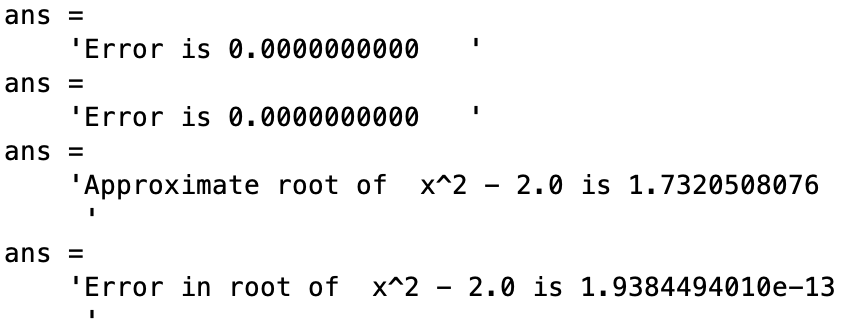
\includegraphics[width=0.8\textwidth]{3bv.png}
\end{figure}

\question
$\alpha$ can be approximated with some iteration errors from Newton's method. It agrees with our prediction that Newton's method has quadratic convergence.
\begin{align*}
	e_{n-1}	&=	0.2036634781	\\
	e_{n}	&=	0.0107140844	\\
	e_{n+1}	&=	0.0000329338	\\
	\alpha	&\approx	\frac{\log(0.0000329338/0.0107140844)}{\log(0.0107140844/0.2036634781)} = 1.96\dots \approx \boxed{2}
\end{align*}


\end{document}
